\chapter{Методы передачи данных канального уровня}

\section{Область действия и характеристики протоколов канального уровня}

Канальный уровень обеспечивает передачу пакетов данных, поступающих от протоколов верхних уровней, узлу назначения, адрес которого также указывает протокол верхнего уровня.
Протоколы канального уровня оформляют переданные им пакеты в кадры собственного формата, помещая указанный адрес назначения в одно из полей такого кадра, а также сопровождая кадр контрольной суммой.

Протокол канального уровня имеет локальный смысл, он предназначен для \emph{доставки кадров данных, как правило, в пределах сетей с простой  топологией связей и однотипной или близкой технологией}, например в односегментных сетях Ethernet или же в многосегментных сетях Ethernet и Token Ring иерархической топологии, разделенных только мостами и коммутаторами.
Во всех этих конфигурациях адрес назначения имеет локальный смысл для данной сети и не изменяется при прохождении кадра от узла-источника к узлу назначения.

Другой областью действия протоколов канального уровня являются \emph{связи типа «точка-точка» глобальных сетей, когда протокол канального уровня ответственен за доставку кадра непосредственному соседу}.
Адрес в этом случае не имеет принципиального значения, а на первый план выходит способность протокола восстанавливать искаженные и утерянные кадры.

Наиболее существенными характеристиками метода передачи, а значит, и протокола, работающего на канальном уровне, являются следующие:
\begin{itemize}
    \item асинхронный/синхронный;
    \item символьно-ориентированный/бит-ориентированный;
    \item с предварительным установлением соединения/дейтаграммный;
    \item с обнаружением искаженных данных/без обнаружения;
    \item с обнаружением потерянных данных/без обнаружения;
    \item с восстановлением искаженных и потерянных данных/без восстановления;
    \item с поддержкой динамической компрессии данных/без поддержки.
\end{itemize}

Многие из этих свойств характерны не только для протоколов канального уровня, но и для протоколов более высоких уровней.

\section{Асинхронные протоколы}

Единицей передаваемых данных в \emph{асинхронных протоколах} изначально был не кадр данных, а отдельный символ (байт со старт-стопными символами).

В асинхронных протоколах применяются стандартные наборы символов, чаще всего ASCII или EBCDIC.
Так как первые 32 или 27 символа в этих наборах являются специальными и не отображаются на дисплее или принтере, то они используются асинхронными протоколами для управления режимом обмена данными.
В самих пользовательских данных, которые представляли собой буквы, цифры, а также такие знаки, как @, \%, \$ и т.
п.
, специальные символы никогда не встречались, так что проблемы их отделения от пользовательских данных не существовало.

Постепенно асинхронные протоколы усложнялись и стали наряду с отдельными символами использовать целые блоки данных, то есть кадры.
При этом, как правило, часть управляющих операций выполнялась посылкой в асинхронном режиме отдельных символов, в то же время часть данных пересылалась блоками, что более характерно для синхронных протоколов.

\section{Синхронные символьно-ориентированные и бит-ориентированные протоколы}

В \emph{синхронных протоколах} все обмены данными осуществляются кадрами, которые имеют в общем случае заголовок, поле данных и концевик.
Все биты кадра передаются непрерывным синхронным потоком, что значительно ускоряет передачу данных.

Кадр1 : (Синхро-биты|Служебная информация|Данные|КС)

Кадр2 : ...

Рисунок 1. Кадры синхронных протоколов

Так как байты в этих протоколах не отделяются друг от друга служебными сигналами, то одной из первых задач приемника является распознавание границы байт.
Затем приемник должен найти начало и конец кадра, а также определить границы каждого поля кадра - адреса назначения, адреса источника, других служебных полей заголовка, поля данных и контрольной суммы.

Большинство протоколов допускает использование в кадре поля данных переменной длины.
Иногда и заголовок может иметь переменную длину.
Обычно протоколы определяют максимальное и, значительно реже, минимальное значение, которое может иметь длина поля данных.
Существуют также протоколы с кадрами фиксированной длины, для которых необходимо решить только первую часть задачи - распознать начало кадра.

\emph{Синхронные протоколы канального уровня} бывают двух типов: \emph{символьно-ориентированные (байт-ориентированные)} и \emph{бит-ориентированные}.
Для обоих характерны одни и те же методы синхронизации бит.
Главное различие между ними заключается в методе синхронизации символов и кадров.

\subsubsection{Символьно-ориентированные протоколы}

Символьно-ориентированные протоколы используются в основном для передачи блоков отображаемых символов, например текстовых файлов.
Так как при синхронной передаче нет стоповых и стартовых битов, для синхронизации символов  передатчик добавляет два или более управляющих символа, называемых символами SYN, перед каждым кадром.
В коде ASCII символ SYN имеет двоичное значение 0010110, это несимметричное относительно начала символа значение позволяет легко разграничивать отдельные символы SYN при их последовательном приеме.

Символы SYN выполняют две функции: во-первых, они обеспечивают приемнику побитную синхронизацию, во-вторых, как только битовая синхронизация достигается, они позволяют приемнику начать распознавание границ символов SYN.

После того как приемник начал отделять один символ от другого, можно задавать границы начала кадра с помощью другого специального символа.
Обычно в символьных протоколах для этих целей используется символ STX (Start of TeXt, ASCII 0000010).
Другой символ отмечает окончание кадра - ETX (End of TeXt, ASCII 0000011).

Однако такой простой способ выделения начала и конца кадра недостаточно хорош, так как внутри кадра (в поле данных) могут встретиться символы STX и ETX.
Для исключения возможности неправильного определения начала и конца кадра предусматриваются два режима - непрозрачный, в котором некоторые специальные символы внутри кадра запрещаются, и прозрачный, в котором разрешается передача внутри кадра любых символов, в том числе и ETX.
Прозрачность достигалась за счет того, что перед символами STX и ETX в поле данных всегда вставлялся символ DLE (Data Link Escape).
Такая процедура называется стаффингом символов (stuff - всякая всячина, заполнитель).
А если в поле данных кадра встречалась последовательность DLE ETX, то передатчик удваивал символ DLE, то есть порождал последовательность DLE DLE ETX.
Приемник, встретив подряд два символа DLE DLE, всегда удалял первый, а оставшиеся символы DLE ETX считал просто пользовательскими данными.

\subsubsection{Бит-ориентированные протоколы}

\emph{Символьно-ориентированная передача} обладает рядом существенных недостатков, ограничивающих ее применение.
Так она не эффективна для передачи двоичных данных, так как приходится в поле данных кадра добавлять достаточно много избыточных данных и, кроме того, формат управляющих символов для разных кодировок различен.

Для того чтобы преодолеть эти проблемы, сегодня при передаче как двоичных, так и символьных данных используется более универсальный метод, называемый \emph{бит-ориентированной передачей}.

Используются три различные схемы бит-ориентированной передачи, отличающиеся способом обозначения начала и конца каждого кадра.

Первая схема \emph{с использованием стартового и стопового флагов}, (верхняя эпюра), похожа на схему с символами STX и ETX в символьно-ориентированных протоколах.
Начало и конец каждого кадра отмечается одной и той же 8-битовой последовательностью - 01111110, называемой флагом.
Термин «бит-ориентированный» используется потому, что принимаемый поток бит сканируется приемником на побитовой основе для обнаружения флага.
Длина кадра в этом случае не обязательно должна быть кратна 8 бит.

Чтобы обеспечить битовую синхронизацию приемника, передатчик посылает последовательность байтов простоя (каждый состоит из 11111111), предшествующую стартовому флагу.

Для достижения прозрачности данных в этой схеме необходимо, чтобы флаг не присутствовал в поле данных кадра.
Это достигается с помощью приема, известного как вставка 0 бита, - бит-стаффинга, которая работает только во время передачи поля данных кадра.
Если эта схема обнаруживает, что подряд передано пять 1, то она автоматически вставляет дополнительный 0 (даже если после этих пяти 1 шел 0).
Поэтому последовательность 01111110 никогда не появится в поле данных кадра.
Аналогичная схема работает в приемнике и выполняет обратную функцию.
Когда после пяти 1 обнаруживается 0, он автоматически удаляется из поля данных кадра.

\begin{figure}
    \centering
    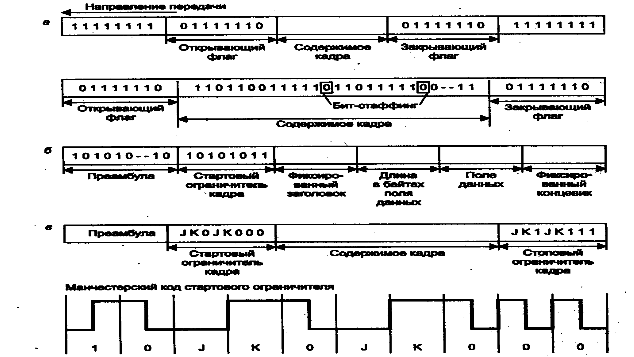
\includegraphics[width=0.9\textwidth]{frame-start-and-stop-marking}
    \caption{Способы выделения начала и конца кадра при синхронной передаче}
    \label{fig:frame-start-and-stop-marking}
\end{figure}

Во второй схеме имеется только \emph{стартовый флаг}, а для определения конца кадра используется \emph{поле длины кадра}.
Эта схема наиболее применима в локальных сетях.
В этих сетях для обозначения факта незанятости среды в исходном состоянии по среде вообще не передается никаких символов.
Чтобы все остальные станции вошли в битовую синхронизацию, посылающая станция предваряет содержимое кадра преамбулой, которая состоит из чередования единиц и нулей 101010...
Войдя в битовую синхронизацию, приемник исследует входной поток на побитовой основе, пока не обнаружит байт начала кадра 10101011.
За этим байтом следует заголовок кадра, в котором имеется поле длины поля данных.
В этой схеме приемник просто отсчитывает заданное количество байт, чтобы определить окончание кадра.

Третья схема использует \emph{для обозначения начала и конца кадра флага}, которые \emph{включают запрещенные для данного кода сигналы} (code violations, V).
Например, при манчестерском кодировании вместо обязательного изменения полярности сигнала в середине тактового интервала уровень сигнала остается неизменным и низким (запрещенный сигнал J) или неизменным и высоким (запрещенный сигнал К).
Начало кадра отмечается последовательностью JK0JK000, а конец - последовательностью JK1JK100.
Этот способ очень экономичен, так как не требует ни бит-стаффинга, ни поля длины, но его недостаток заключается в зависимости от принятого метода физического кодирования.

При использовании избыточных кодов роль сигналов J и К играют запрещенные символы (комбинации), например, в коде 4В/5В этими символами являются коды 11000 и 10001.

Каждая из трех схем имеет свои преимущества и недостатки.
Флаги позволяют отказаться от специального дополнительного поля, но требуют специальных мер: либо по разрешению размещения флага в поле данных за счет бит-стаффинга, либо по использованию в качестве флага запрещенных сигналов, что делает эту схему зависимой от способа кодирования.

\subsubsection{Бит-ориентированные протоколы с гибким форматом кадра}

Для большей части протоколов характерны кадры, состоящие из служебных полей фиксированной длины.
Однако существует ряд протоколов, в которых кадры имеют гибкую структуру.
Кадры таких протоколов состоят из неопределенного количества полей, каждое из которых может иметь переменную длину.
Каждое поле обычно описывается двумя дополнительными полями фиксированного размера.
Например, если в кадре встречается поле, содержащее некоторую символьную строку, то в кадр вставляются три поля:

\begin{table}[]
    \begin{tabular}{|l|l|l|}
        \hline
        \textbf{Тип} & \textbf{Длина}         & \textbf{Значение} \\ \hline
        string       & \multicolumn{1}{c|}{6} & public            \\ \hline
    \end{tabular}
\end{table}

Дополнительные поля «Тип» и «Длина» имеют фиксированный размер в один  байт, поэтому протокол легко находит границы поля «Значение».
Так как количество таких полей также неизвестно, для определения общей длины кадра используется либо общее поле «Длина», которое помещается в начале кадра и относится ко всем полям данных, либо закрывающий флаг.

\section{Передача с установлением соединения и без установления соединения}

При передаче кадров данных на канальном уровне используются как \emph{дейтаграммные процедуры}, работающие \emph{без установления соединения (connectionless)}, так и \emph{процедуры с предварительным установлением логического соединения (connection-oriented)}.

\subsubsection{Дейтаграммная передача}

При \emph{дейтаграммной передаче} кадр посылается в сеть «без предупреждения», и никакой ответственности за его утерю протокол не несет.
Предполагается, что сеть всегда готова принять кадр от конечного узла.
Дейтаграммный метод работает быстро, так как никаких предварительных действий перед отправкой данных не выполняется.
Однако при таком методе трудно организовать в рамках протокола отслеживание факта доставки кадра узлу назначения.
Этот метод не гарантирует доставку пакета.

\begin{figure}
    \centering
    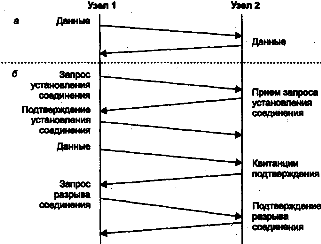
\includegraphics[width=0.6\textwidth]{protocols}
    \caption{Протоколы без установления соединения (а) и с установлением соединения (б)}
    \label{fig:protocols}
\end{figure}

\subsubsection{Передача с установлением соединения}

Передача с установлением соединения более надежна, но требует больше времени для передачи данных и вычислительных затрат от конечных узлов.
При передаче с установлением соединения можно выделить следующие этапы.
\begin{enumerate}
    \item Узел-инициатор отправляет узлу-получателю служебный кадр специального формата с предложением установить соединение.
    \item Если узел-получатель согласен с этим, то он посылает в ответ другой служебный кадр, подтверждающий установление соединения и предлагающий для данного логического соединения некоторые параметры обмена.
К таким параметрам могут относиться идентификатор соединения, максимальное значение поля данных кадров, которые будут использоваться в рамках данного соединения, и т.п.
    \item Узел-инициатор соединения может завершить процесс установления соединения отправкой еще одного служебного кадра, в котором сообщит, что предложенные параметры ему подходят.
    \item На этом этапе логическое соединение считается установленным, и в его рамках можно передавать информационные кадры с пользовательскими данными.
    \item После передачи некоторого законченного набора данных, например определенного файла, узел инициирует разрыв данного логического соединения, посылая соответствующий служебный кадр.
\end{enumerate}

Заметим, что, в отличие от протоколов дейтаграммного типа, которые поддерживают только один тип кадра - информационный, протоколы, работающие по процедуре с установлением соединения, должны поддерживать несколько типов кадров - служебные, для установления (и разрыва) соединения, и информационные, переносящие собственно пользовательские данные.

\section{Обнаружение и коррекция ошибок}

Канальный уровень должен \emph{обнаруживать} ошибки передачи данных, связанные с \emph{искажением бит} в принятом кадре данных или с \emph{потерей кадра} и, \emph{по возможности, их корректировать}.

Большая часть протоколов канального уровня выполняет только первую задачу - обнаружение ошибок, считая, что корректировать ошибки, то есть повторно передавать данные, содержавшие искаженную информацию, должны протоколы верхних уровней.
Так работают такие популярные протоколы локальных сетей, как Ethernet, Token Ring, FDDI и другие.
Однако существуют протоколы канального уровня, например LLC2 или LAP-B, которые самостоятельно решают задачу восстановления искаженных или потерянных кадров.

Очевидно, что протоколы должны работать наиболее эффективно в типичных условиях работы сети.
Поэтому для сетей, в которых искажения и потери кадров являются редкими событиями, разрабатываются протоколы типа Ethernet, в которых не предусматриваются процедуры устранения ошибок.
Напротив, если в сети искажения и потери случаются часто, то желательно уже на канальном уровне использовать протокол с коррекцией ошибок, а не оставлять эту работу протоколам верхних уровней.
Протоколы верхних уровней, например транспортного или прикладного, восстановят потерянные данные с большой задержкой.
В глобальных сетях первых поколений, например сетях Х.
25, которые работали через ненадежные каналы связи, протоколы канального уровня всегда выполняли процедуры восстановления потерянных и искаженных кадров.

\subsubsection{Методы обнаружения ошибок}

Все \emph{методы обнаружения ошибок} основаны на передаче в составе кадра данных избыточной информации, по которой можно судить о достоверности принятых данных.
Эту служебную информацию принято называть контрольной суммой (или последовательностью контроля кадра - Frame Check Sequence, FCS).
Контрольная сумма вычисляется как функция от основной информации, принимающая сторона повторно вычисляет контрольную сумму кадра по известному алгоритму и в случае ее совпадения с контрольной суммой, вычисленной передающей стороной, делает вывод о том, что данные были переданы через сеть корректно.

Существует несколько распространенных алгоритмов вычисления контрольной суммы, отличающихся вычислительной сложностью и способностью обнаруживать ошибки в данных.

\emph{Контроль по паритету} представляет собой наиболее простой и наименее мощный алгоритм контроля, так как с его помощью можно обнаружить только одиночные ошибки в проверяемых данных.
Метод заключается в суммировании по модулю 2 всех бит контролируемой информации.
Например, для данных 100101011 результатом контрольного суммирования будет значение 1.
Результат суммирования также представляет собой один бит данных, который пересылается вместе с контролируемой информацией.
При искажении в ходе пересылки любого одного бита исходных данных, в том числе контрольного разряда результат суммирования будет отличаться от принятого контрольного разряда, что говорит об ошибке.
Однако двойная ошибка, например 110101010, будет неверно принята за корректные данные.
Поэтому контроль по паритету применяется к небольшим порциям данных, как правило, к каждому байту, что дает коэффициент избыточности для этого метода 1/8.
Метод редко применяется в вычислительных сетях из-за его большой избыточности и невысоких диагностических способностей.

\emph{Вертикальный и горизонтальный контроль} по паритету представляет собой модификацию описанного выше метода.
Его отличие состоит в том, что исходные данные рассматриваются в виде матрицы, строки которой составляют байты данных.
Контрольный разряд подсчитывается отдельно для каждой строки и для каждого столбца матрицы.
Этот метод обнаруживает большую часть двойных ошибок, однако обладает еще большей избыточностью.
На практике сейчас также почти не применяется.

\emph{Циклический избыточный контроль (Cyclic Redundancy Check, CRC)} является в настоящее время наиболее популярным методом контроля в вычислительных сетях.
Метод основан на рассмотрении исходных данных в виде одного многоразрядного двоичного числа.
Например, кадр стандарта Ethernet, состоящий из 1024 байт, будет рассматриваться как одно число, состоящее из 8192 бит.
В качестве контрольной информации рассматривается остаток от деления этого числа на известный делитель R.
Обычно в качестве делители выбирается семнадцати- или тридцатитрехразрядное число, чтобы остаток от деления имел длину 16 разрядов (2 байт) или 32 разряда (4 байт).
При получении кадра данных снова вычисляется остаток от деления на тот же делитель R, но при этом к данным кадра добавляется и содержащаяся в нем контрольная сумма.
Если остаток от деления на R равен нулю, то делается вывод об отсутствии ошибок в полученном кадре
Этот метод обладает более высокой вычислительной сложностью, но его диагностические возможности гораздо выше, чем у методов контроля по паритету.
Метод CRC обнаруживает все одиночные ошибки, двойные ошибки и ошибки в нечетном числе бит.
Метод обладает также невысокой степенью избыточности.
Например, для кадра Ethernet размером в 1024 байт контрольная информация длиной в 4 байт составляет только 0,4 %.

\subsubsection{Методы восстановления искаженных и потерянных кадров}

\emph{Методы коррекции ошибок} в вычислительных сетях \emph{основаны на повторной передаче кадра} в тех случаях, если кадр теряется и не доходит до адресата или приемник обнаружил в нем искажение информации.
Чтобы убедиться в необходимости повторной передачи данных, отправитель нумерует отправляемые кадры и для каждого кадра ожидает от приемника так называемой положительной квитанции - служебного кадра, извещающего о том, что исходный кадр был получен и данные в нем оказались корректными.
Время этого ожидания ограничено - при отправке каждого кадра передатчик запускает таймер, и, если по его истечении положительная квитанция не получена, кадр считается утерянным.
Приемник в случае получения кадра с искаженными данными может отправить отрицательную квитанцию - явное указание на то, что данный кадр нужно передать повторно.

Существуют два подхода к организации процесса обмена квитанциями - \emph{с простоями (с ожиданием подтверждения)} и \emph{с организацией «окна» (метод скользящего окна)}, принцип взаимодействия абонентов при реализации этих подходов иллюстрируется рисунком.

\begin{figure}
    \centering
    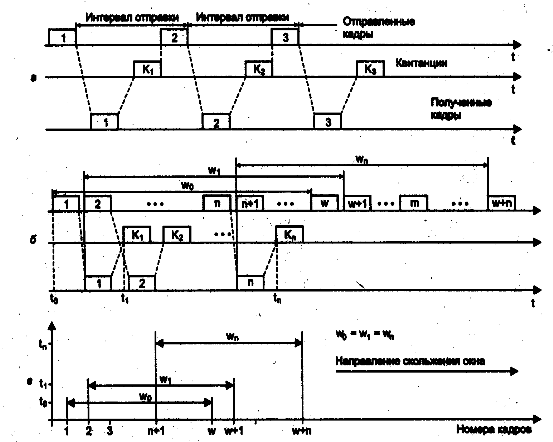
\includegraphics[width=0.9\textwidth]{frames-restoration-methods}
    \caption{Методы восстановления искаженных и потерянных кадров}
    \label{fig:frames-restoration-methods}
\end{figure}

\emph{Метод с простоями (Idle Source)} требует, чтобы источник, пославший кадр, ожидал получения квитанции (положительной или отрицательной) от приемника и только после этого посылал следующий кадр (или повторял искаженный).
Если же квитанция не приходит в течение тайм-аута, то кадр (или квитанция) считается утерянным и его передача повторяется.
В этом случае производительность обмена данными существенно снижается, - хотя передатчик и мог бы послать следующий кадр сразу же после отправки предыдущего, он обязан ждать прихода квитанции.
Снижение производительности этого метода коррекции особенно заметно на низкоскоростных каналах связи, то есть в территориальных сетях.

Второй метод называется методом \emph{скользящего окна (Sliding Window)}.
В этом методе для повышения коэффициента использования линии источнику разрешается передать некоторое количество кадров в непрерывном режиме, то есть в максимально возможном для источника темпе, без получения на эти кадры положительных ответных квитанций.
Количество кадров, которые разрешается передать таким образом, называется размером окна.
Рисунок иллюстрирует данный метод для окна размером в $W$ кадров.

В начальный момент, когда еще не послано ни одного кадра, окно определяет диапазон кадров с номерами от $1$ до $W$ включительно.
Источник начинает передавать кадры и получать в ответ квитанции.
Для простоты предположим, что квитанции поступают в той же последовательности, что и кадры, которым они соответствуют.
В момент $t_1$ при получении первой квитанции $K_1$ окно сдвигается на одну позицию, определяя новый диапазон от $2$ до $(W + 1)$.

Процессы отправки кадров и получения квитанций идут достаточно независимо друг от друга.
Рассмотрим произвольный момент времени $t_n$, когда источник получил квитанцию на кадр с номером $n$.
Окно сдвинулось вправо и определило диапазон разрешенных к передаче кадров от $(n + 1)$ до $(W + n)$.
Все множество кадров, выходящих из источника, можно разделить на перечисленные ниже группы (рис. \ref{fig:frame-restoration-methods}).
\begin{itemize}
    \item
        Кадры с номерами от $1$ до $n$ уже были отправлены и квитанции на них получены, то есть они находятся за пределами окна слева.

    \item
        Кадры, начиная с номера $(n + 1)$ и кончая номером $(n + W)$, находятся в пределах.
окна и потому могут быть отправлены не дожидаясь прихода какой-либо квитанции.
        Этот диапазон может быть разделен еще на два поддиапазона:
        \begin{itemize}
            \item кадры с номерами от $(n + 1)$ до $m$, которые уже отправлены, но квитанции на них еще не получены;
            \item кадры с номерами от $m$ до $(n + W)$, которые пока не отправлены, хотя запрета на это нет.
        \end{itemize}
    \item
        Все кадры с номерами, большими или равными $(n + W + 1)$, находятся за пределами окна справа и поэтому пока не могут быть отправлены.
\end{itemize}

Метод скользящего окна более сложен в реализации, чем метод с простоями, так как передатчик должен хранить в буфере все кадры, на которые пока не получены положительные квитанции.
Кроме того, требуется отслеживать несколько параметров алгоритма: размер окна $W$, номер кадра, на который получена квитанция, номер кадра, который еще можно передать до получения новой квитанции.

Метод скользящего окна имеет два параметра, которые могут заметно влиять на эффективность передачи данных между передатчиком и приемником, - размер окна и величина тайм-аута ожидания квитанции.
В надежных сетях, когда кадры искажаются и теряются редко, для повышения скорости обмена данными размер окна можно увеличивать, так как при этом передатчик будет посылать кадры с меньшими паузами.
В ненадежных сетях размер окна следует уменьшать, так как при частых потерях и искажениях кадров резко возрастает объем вторично передаваемых через сеть кадров, а значит, пропускная способность сети будет расходоваться во многом вхолостую - полезная пропускная способность сети будет падать.

Выбор тайм-аута зависит не от надежности сети, а от задержек передачи кадров сетью.

Во многих реализациях метода скользящего окна величина окна и тайм-аут выбираются адаптивно, в зависимости от текущего состояния сети.

\section{Компрессия данных}

\emph{Компрессия (сжатие) данных} применяется для сокращения времени их передачи.
Так как на компрессию данных передающая сторона тратит дополнительное время, к которому нужно еще прибавить аналогичные затраты времени на декомпрессию этих данных принимающей стороной, то выгоды от сокращения времени на передачу сжатых данных обычно бывают заметны только для низкоскоростных каналов.
Этот порог скорости для современной аппаратуры составляет около 64 Кбит/с.

На практике может использоваться ряд алгоритмов компрессии, каждый из которых применим к определенному типу данных.
Некоторые модемы (называемые интеллектуальными) предлагают адаптивную компрессию, при которой в зависимости от передаваемых данных выбирается определенный алгоритм компрессии.
Рассмотрим некоторые из общих алгоритмов компрессии данных.

\emph{Десятичная упаковка}.
Когда данные состоят только из чисел, значительную экономию можно получить путем уменьшения количества используемых на цифру бит с 7 до 4, используя простое двоичное кодирование десятичных цифр вместо кода ASCII.

\emph{Относительное кодирование}.
Альтернативой десятичной упаковке при передаче числовых данных с небольшими отклонениями между последовательными отсчетами является передача только этих отклонений вместе с известным опорным значением.
Такой метод используется, в частности, в методе цифрового кодирования голоса, передающем в каждом такте только разницу между соседними замерами голоса.

\emph{Символьное подавление}.
Часто передаваемые данные содержат большое количество повторяющихся байт (например, при передаче черно-белого изображения).
Передатчик сканирует последовательность передаваемых байт и, если обнаруживает последовательность из трех или более одинаковых байт, заменяет ее специальной трехбайтовой последовательностью, в которой указывает значение байта, количество его повторений, а также отмечает начало этой последовательности специальным управляющим символом.

\emph{Коды переменной длины}.
В этом методе кодирования используется тот факт, что не все символы в передаваемом кадре встречаются с одинаковой частотой.
Поэтому во многих схемах кодирования коды часто встречающихся символов заменяют кодами меньшей длины, а редко встречающихся - кодами большей длины.

\emph{При статистическом кодировании} коды выбираются таким образом, чтобы при анализе последовательности бит можно было бы однозначно определить соответствие определенной порции бит тому или иному символу или же запрещенной комбинации бит.
Если данная последовательность бит представляет собой запрещенную комбинацию, то необходимо к ней добавить еще один бит и повторить анализ.
Например, если при неравномерном кодировании для наиболее часто встречающегося символа «Р» выбран код 1, состоящий из одного бита, то значение 0 однобитного кода будет запрещенным.
Иначе мы сможем закодировать только два символа.
Для другого часто встречающегося символа «О» можно использовать код 01, а код 00 оставить как запрещенный.

Неравномерное кодирование наиболее эффективно, когда неравномерность распределения частот передаваемых символов достаточна велика, как при передаче длинных текстовых строк.
Напротив, при передаче двоичных данных, например кодов программ, оно малоэффективно, так как 8-битовые коды при этом распределены почти равномерно.

Многие модели коммуникационного оборудования, такие как модемы, мосты, коммутаторы и маршрутизаторы, поддерживают протоколы динамической компрессии, позволяющие сократить объем передаваемой информации в 4, а иногда и в 8 раз.
В таких случаях говорят, что протокол обеспечивает коэффициент сжатия 1:4 или 1:8.
Существуют стандартные протоколы компрессии, например V.
42bis, a также большое количество нестандартных, фирменных протоколов.
Реальный коэффициент компрессии зависит от типа передаваемых данных, так, графические и текстовые данные обычно сжимаются хорошо, а коды программ - хуже.

\section{Методы коммутации}

\subsection{Понятие о коммутируемых сетях}

В связи с тем, что практически невозможно предоставить каждой паре взаимодействующих абонентов свою собственную некоммутируемую физическую линию связи в любой сети всегда применяется какой-либо способ коммутации абонентов, который обеспечивает доступность имеющихся физических каналов одновременно для нескольких сеансов связи между абонентами сети.

Существуют три принципиально различные схемы коммутации абонентов в сетях:
\begin{itemize}
    \item \emph{коммутация каналов (circuit switching)};
    \item \emph{коммутация пакетов (packet switching)};
    \item \emph{коммутация сообщений (message switching)}.
\end{itemize}

Как сети с коммутацией пакетов, так и сети с коммутацией каналов можно разделить на два класса по другому признаку - на сети с динамической коммутацией и сети с постоянной коммутацией

\subsection{Коммутация каналов}

Коммутация каналов подразумевает образование непрерывного составного физического канала из последовательно соединенных отдельных канальных участков для прямой передачи данных между узлами.
Отдельные каналы соединяются между собой специальной аппаратурой - коммутаторами, которые могут устанавливать связи между любыми конечными узлами сети.
В сети с коммутацией каналов перед передачей данных всегда необходимо выполнить процедуру установления соединения, в процессе которой и создается составной канал.

Например, если сеть, рассмотренная нами выше, работает по технологии коммутации каналов, то узел 1, чтобы передать данные узлу 7, прежде всего должен передать специальный запрос на установление соединения коммутатору A, указав адрес назначения 7.
Коммутатор A должен выбрать маршрут образования составного канала, а затем передать запрос следующему коммутатору, в данном случае E.
Затем коммутатор E передает запрос коммутатору F, а тот, в свою очередь, передает запрос узлу 7.
Если узел 7 принимает запрос на установление соединения, он направляет по уже установленному каналу ответ исходному узлу, после чего составной канал считается скоммутированным, и узлы 1 и 7 могут обмениваться по нему данными, например, вести телефонный разговор.

Коммутаторы, а также соединяющие их каналы должны обеспечивать одновременную передачу данных нескольких абонентских каналов.
Для этого они должны быть высокоскоростными и поддерживать какую-либо технику мультиплексирования абонентских каналов.

В настоящее время \emph{для мультиплексирования абонентских каналов} используются две техники:
\begin{itemize}
    \item \emph{техника частотного мультиплексирования (Frequency Division Multiplexing, FDM)};
    \item \emph{техника мультиплексирования с разделением времени (Time Division Multiplexing, TDM)}.
\end{itemize}

\subsection{Принцип коммутации пакетов}

\emph{Коммутация пакетов} - это техника коммутации абонентов, которая была специально разработана для эффективной передачи компьютерного трафика.
Коэффициент пульсации трафика отдельного пользователя сети, равный отношению средней интенсивности обмена данными к максимально возможной, может составлять 1:50 или 1:100.
Если организовать коммутацию канала между компьютером пользователя и сервером, то большую часть времени канал будет простаивать.
В то же время часть тайм-слотов или частотных полос коммутаторов будет занята и недоступна другим пользователям сети.

При коммутации пакетов все передаваемые пользователем сети сообщения разбиваются в исходном узле на сравнительно небольшие части, называемые пакетами.
Напомним, что сообщением называется логически завершенная порция данных - запрос на передачу файла, ответ на этот запрос, содержащий весь файл, и т.п.
Сообщения могут иметь произвольную длину, от нескольких байт до многих мегабайт.
Напротив, пакеты обычно тоже могут иметь переменную длину, но в узких пределах, например от 46 до 1500 байт.
Каждый пакет снабжается заголовком, в котором указывается адресная информация, необходимая для доставки пакета узлу назначения, а также номер пакета, который будет использоваться узлом назначения для сборки сообщения (рис. \ref{fig:packet-breaking}).
Пакеты транспортируются в сети как независимые информационные блоки.
Коммутаторы сети принимают пакеты от конечных узлов и на основании адресной информации передают их друг другу, а в конечном итоге - узлу назначения.

\begin{figure}
    \centering
    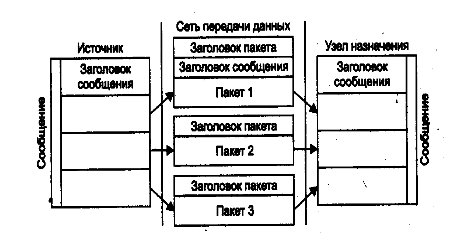
\includegraphics[width=0.8\textwidth]{packet-breaking}
    \caption{Разбиение сообщения на пакеты}
    \label{fig:packet-breaking}
\end{figure}

Коммутаторы пакетной сети отличаются от коммутаторов каналов тем, что они имеют внутреннюю буферную память для временного хранения пакетов, в случае если выходной порт коммутатора в момент принятия пакета занят передачей другого пакета.
В этом случае пакет находится некоторое время в очереди пакетов в буферной памяти выходного порта, а когда до него дойдет очередь, то он передается следующему коммутатору.
Такая схема передачи данных позволяет сглаживать пульсации трафика на магистральных связях между коммутаторами.

Существует и другой режим работы сети - передача пакетов по \emph{виртуальному каналу (virtual circuit или virtual channel)}.
В этом случае перед тем, как начать передачу данных между двумя конечными узлами, должен быть установлен виртуальный канал, который представляет собой единственный маршрут, соединяющий эти конечные узлы.
Виртуальный канал может быть динамическим или постоянным.

При отказе коммутатора или канала на пути виртуального канала соединение разрывается, и виртуальный канал нужно прокладывать заново.
При этом он, естественно, обойдет отказавшие участки сети.

\subsection{Коммутация сообщений}

Под \emph{коммутацией сообщений} понимается передача единого блока данных между транзитными компьютерами сети с временной буферизацией этого блока на диске каждого компьютера.
Сообщение в отличие от пакета имеет произвольную длину, которая определяется не технологическими соображениями, а содержанием информации, составляющей сообщение.
Например, сообщением может быть текстовый документ, файл с кодом программы, электронное письмо.

Транзитные компьютеры могут соединяться между собой как сетью с коммутацией пакетов, так и сетью с коммутацией каналов.
Сообщения хранятся в транзитном компьютере на диске, причем время хранения может быть достаточно большим, если компьютер загружен другими работами или сеть временно перегружена.

По такой схеме обычно передаются сообщения, не требующие немедленного ответа, чаще всего сообщения электронной почты.
Режим передачи с промежуточным хранением на диске называется режимом \emph{<<хранение-и-передача>> (store-and-forward)}.

Режим коммутации сообщений разгружает сеть для передачи трафика, требующего быстрого ответа, например графика службы WWW или файловой службы.
Количество транзитных компьютеров стараются по возможности уменьшить.
Если компьютеры подключены к сети с коммутацией пакетов, то число промежуточных компьютеров обычно уменьшается до двух.
Например, пользователь передает почтовое сообщение своему серверу исходящей почты, а тот сразу старается передать сообщение серверу входящей почты адресата.
Но если компьютеры связаны между собой телефонной сетью, то часто используется несколько промежуточных серверов, так как прямой доступ к конечному серверу может быть невозможен в данный момент из-за перегрузки телефонной сети (абонент занят) или экономически невыгоден из-за высоких тарифов на дальнюю телефонную связь.

Техника коммутации сообщений появилась в компьютерных сетях раньше техники коммутации пакетов, но потом была вытеснена последней, как более эффективной по критерию пропускной способности сети.
Запись сообщения на диск занимает достаточно много времени, кроме того, наличие дисков предполагает специализированные компьютеры в качестве коммутаторов, что удорожает сеть.

Сегодня коммутация сообщений работает только для некоторых не оперативных служб, причем чаще всего поверх сети с коммутацией пакетов, как служба прикладного уровня

